\documentclass{beamer}
\usetheme{Madrid}

\usepackage{amsmath, amssymb, amsthm}
\usepackage{graphicx}
\usepackage{listings}
\usepackage{gensymb}
\usepackage[utf8]{inputenc}
\usepackage{hyperref}
\usepackage{tikz}
\lstset{
  language=Python,
  basicstyle=\ttfamily\small,
  keywordstyle=\color{blue},
  stringstyle=\color{orange},
  numbers=left,
  numberstyle=\tiny\color{gray},
  breaklines=true,
  showstringspaces=false
}
\usetikzlibrary{decorations.pathmorphing}

\title{Question-12.9.7.1.1}
\author{EE24BTECH11030 - J.KEDARANANDA}
\date{}
\begin{document}

\frame{\titlepage}

\begin{frame}
\frametitle{Question}
Solve the differential equation:
\begin{align}
    \frac{d^2y}{dx^2} + 5x \left( \frac{dy}{dx} \right)^2 - 6y = \ln(x),
\end{align}
\end{frame}

\begin{frame}
\frametitle{Theoritical Solution : }

\centering
The given differential equation is a second-order nonlinear ordinary differential equation
and cannot be theoritcally solved using known methods.
\end{frame}

\begin{frame}
\frametitle{Computational Solution : }
Euler's Method
\textbf{By the first principle of derivative,}
\begin{align}
    y^{\prime}(x) &= \lim_{h\to0} \frac{y(x + h) - y(x)}{h}\\
    y(x + h) &= y(x) + h \cdot y^{\prime}(x), \quad h\to0
\end{align}

\textbf{For a $m^{\text{th}}$ order differential equation:}

\medskip

Let:
\begin{align}
    y_1 = y, \quad y_2 = y^{\prime}, \quad y_3 = y^{\prime\prime}, \quad \dots, \quad y_m = y^{m - 1}
\end{align}
\end{frame}
\begin{frame}{Euler's Method (System of Equations)}
\textbf{Then, we obtain the system:}
\begin{align}
    \begin{bmatrix}
        y_1^{\prime} \\ 
        y_2^{\prime} \\ 
        \vdots \\ 
        y_{m - 1}^{\prime} \\ 
        y_m^{\prime}
    \end{bmatrix}
    =
    \begin{bmatrix}
        y_2 \\ 
        y_3 \\ 
        \vdots \\ 
        y_m \\ 
        f(x, y_1, y_2, \dots, y_m)
    \end{bmatrix}
\end{align}

Here, $f$ is described by the given differential equation.

\medskip

The initial conditions are:
\begin{align*}
    y_1(x_0) = K_1, \quad 
    y_2(x_0) = K_2, \quad 
    \dots, \quad 
    y_m(x_0) = K_m
\end{align*}
\end{frame}
\begin{frame}{Euler's Method (System Representation)}
\textbf{Representing the system in Euler's form (using the first principle of derivative):}
\begin{align}
    \begin{bmatrix}
        y_1(x + h) \\ 
        y_2(x + h) \\ 
        \vdots \\ 
        y_m(x + h)
    \end{bmatrix}
    &=
    \begin{bmatrix}
        y_1(x) + h y_2(x) \\ 
        y_2(x) + h y_3(x) \\ 
        \vdots \\ 
        y_m(x) + h f(x, y_1, y_2, \dots, y_m)
    \end{bmatrix}\\
    \begin{bmatrix}
        y_1(x+h) \\ 
        \vdots \\ 
        y_{m-1}(x+h) \\ 
        y_m(x+h)
    \end{bmatrix}
    &=
    \begin{bmatrix}
        y_1(x) \\ 
        \vdots \\ 
        y_{m-1}(x) \\ 
        y_m(x)
    \end{bmatrix}
    +
    h
    \begin{bmatrix}
        y_2(x) \\ 
        \vdots \\ 
        y_m(x) \\ 
        f(x, y_1, y_2, \dots, y_m)
    \end{bmatrix}
\end{align}
\end{frame}
\begin{frame}{Euler's Method (System Representation)}
\begin{align}
    \vec{y}(x+h) 
    &=
    \vec{y}(x) 
    +
    h
    \begin{bmatrix}
        0 & 1 & 0 & 0 & \dots & 0 & 0 \\
        0 & 0 & 1 & 0 & \dots & 0 & 0 \\
        0 & 0 & 0 & 1 & \dots & 0 & 0 \\
        \vdots & \vdots & \vdots & \vdots & \ddots & \vdots & \vdots \\
        0 & 0 & 0 & 0 & \dots & 0 & 1 \\
        0 & 0 & 0 & 0 & \dots & 0 & \frac{f(x, y_1, y_2, \dots, y_m)}{y_m}
    \end{bmatrix}
    \vec{y}(x) \\
    \vec{y}(x+h) 
    &=
    \begin{bmatrix}
        1 & h & 0 & 0 & \dots & 0 & 0 \\
        0 & 1 & h & 0 & \dots & 0 & 0 \\
        0 & 0 & 1 & h & \dots & 0 & 0 \\
        \vdots & \vdots & \vdots & \vdots & \ddots & \vdots & \vdots \\
        0 & 0 & 0 & 0 & \dots & 1 & h \\
        0 & 0 & 0 & 0 & \dots & 0 & 1+\frac{f(x, y_1, y_2, \dots, y_m)}{y_m}
    \end{bmatrix}
    \vec{y}(x)
\end{align}
\end{frame}
\begin{frame}{System Representation for a Specific Differential Equation (Part 1)}
\textbf{Note:} The vector $\vec{y_n}$ is not to be confused with $y_k$, which represents the $(k-1)^{\text{th}}$ derivative of $y(x)$.

\medskip

The given differential equation is:
\begin{align}
    y^{\prime\prime} + 5x(y^{\prime})^2 - 6y &= \ln(x) \\
    y^{\prime\prime} &= \ln(x) - 5x(y^{\prime})^2 + 6y
\end{align}

We see that $m = 2$, so:
\begin{align}
    y_3 &= y^{\prime\prime} = \ln(x) - 5x(y^{\prime})^2 + 6y \\
    \begin{bmatrix}
        y_1^{\prime} \\ 
        y_2^{\prime}
    \end{bmatrix}
    &=
    \begin{bmatrix}
        y_2 \\ 
        \ln(x) - 5x(y^{\prime})^2 + 6y
    \end{bmatrix}
\end{align}
\end{frame}
\begin{frame}{System Representation for a Specific Differential Equation (Part 2)}
\textbf{Iterative System Representation:}
\begin{align}
    \begin{bmatrix}
        y_{1, n+1} \\ 
        y_{2, n+1}
    \end{bmatrix}
    &=
    \begin{bmatrix}
        y_{1, n} \\ 
        y_{2, n}
    \end{bmatrix}
    +
    h
    \begin{bmatrix}
        y_{2, n} \\ 
        \ln(x_n) - 5x_n(y_{2,n})^2 + 6y_{1,n}
    \end{bmatrix} \\
    \vec{y}_{n+1} &= 
    \begin{bmatrix}
        1 & h \\ 
        0 & 1 + \ln(x_n) - 5x_n(y_{2,n})^2 + 6y_{1,n}
    \end{bmatrix}
    \vec{y}_n
\end{align}

\textbf{Initial Conditions:}
\begin{align}
    x_0 = 0, \quad y_{1, 0} = 0.01, \quad y_{2, 0} = 1
\end{align}
\end{frame}
\begin{frame}
\frametitle{Diagram}
\begin{figure}[!ht]
    \centering
    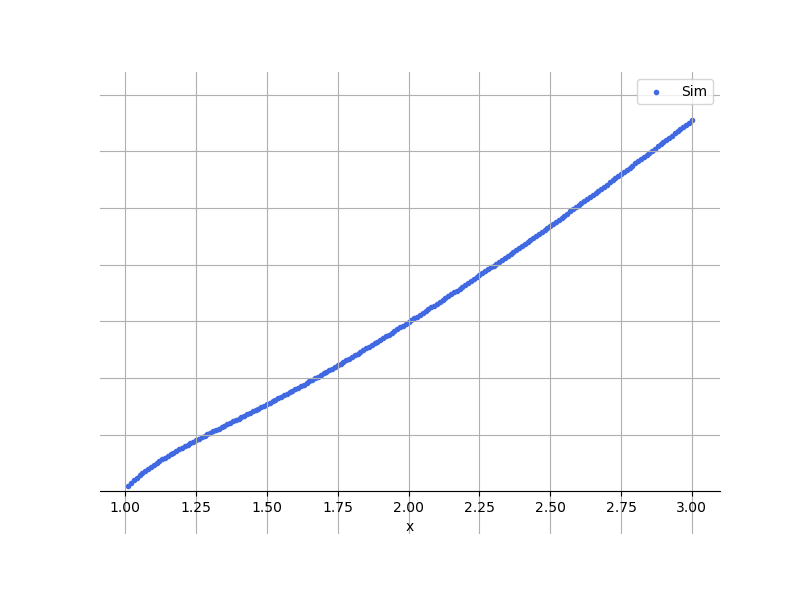
\includegraphics[width=\linewidth]{figs/Fig.png}
    \caption{Ellipse bounded region}
\end{figure}
\end{frame}

\begin{frame}[fragile]
\frametitle{C-Code}
\begin{lstlisting}[language=C]
#include <stdlib.h>
#include <math.h>

// get 'n' points on the plot of the differential equation, 'h' being the step size, 'x', 'y1', 'y2' being the inital conditions
// y1 = y, y2 = y'
float **diffEqPoints(int n, float h, float x, float y1, float y2){
  float pts = (float ) malloc(sizeof(float *) * n);

  // iteratively use euler's method with given parameters to return 'n' points in the plot of the differential equation
  for (int i = 0; i < n; i++){
    pts[i] = (float *) malloc(sizeof(float) * 2);
\end{lstlisting}
\end{frame}
\begin{frame}[fragile]
\frametitle{C-Code}
    \begin{lstlisting}[language=C]
           float y2_new = y2 + h*(-5 * x * pow(y2, 2) + 6 * y1 + log(x));
    y1 = y1 + h*y2;
    y2 = y2_new;
    x = x + h;
    pts[i][0] = x;
    pts[i][1] = y1;
  }
  return pts;
}
void freeMultiMem(float **points, int n){
  for(int i = 0; i < n; i++){
    free(points[i]);
  }
  free(points);
}
    \end{lstlisting}
\end{frame}
\begin{frame}[fragile]
\frametitle{Python-Code}
\begin{lstlisting}
import numpy as np
import matplotlib.pyplot as plt
import ctypes
import math

# dll linking
dll = ctypes.CDLL('./points.so')

# describing the argument and return types of the function 'diffEqPoints' and 'freeMultiMem' in the dll
dll.diffEqPoints.argtypes = [ctypes.c_int] + [ctypes.c_float]*4
dll.diffEqPoints.restype = ctypes.POINTER(ctypes.POINTER(ctypes.c_float))

dll.freeMultiMem.argtypes = [ctypes.POINTER(ctypes.POINTER(ctypes.c_float)), ctypes.c_int]
\end{lstlisting}
\end{frame}
\begin{frame}[fragile]
\frametitle{Python-Code}
\begin{lstlisting}
dll.freeMultiMem.restype = None

n = 200  # number of points to plot for given differential equation plot
h = 0.01 # step size

# initial conditions, y1 = y, y2 = dy/dx
x = 1.0    # x must be greater than 0 for log(x)
y1 = 0.01  # initial y1
y2 = 1.0   # initial dy/dx

# setting up the plot
plt.figure(figsize=(8, 6))

# getting an array of all the points in the plot
pts = dll.diffEqPoints(n, h, x, y1, y2)

# plotting the differential equation using plt.scatter
coords = []

\end{lstlisting}
\end{frame}

\begin{frame}[fragile]
\frametitle{Python-Code}
\begin{lstlisting}
for i in range(n):
    pt = pts[i]  # access individual point from the pointer
    print(pt[0], pt[1])  # print coordinates to the console for verification
    coords.append(np.array([pt[0], pt[1]]))

coords_plot = np.array(coords)
plt.scatter(coords_plot[:, 0], coords_plot[:, 1], marker=".", label="Sim", color="royalblue")

# freeing the memory of the array 'pts'
dll.freeMultiMem(pts, n)

# customize the plot (axes, labels, grid)
ax = plt.gca()
ax.spines['top'].set_color('none')
ax.spines['left'].set_position('zero')

\end{lstlisting}
\end{frame}
\begin{frame}[fragile]
\frametitle{Python-Code}
\begin{lstlisting}
ax.spines['right'].set_color('none')
ax.spines['bottom'].set_position('zero')

plt.legend(loc='best')
plt.grid()
plt.axis('equal')

plt.xlabel('x')
plt.ylabel('y')

# Display the plot
plt.show()
\end{lstlisting}
\end{frame}
\end{document}

